
\documentclass{article}
\usepackage{spconf,amsmath,epsfig}
\usepackage{subfigure}

\let\OLDthebibliography\thebibliography
\renewcommand\thebibliography[1]{
  \OLDthebibliography{#1}
  \setlength{\parskip}{0pt}
  \setlength{\itemsep}{0pt plus 0.3ex}
}

\pagestyle{empty}


\begin{document}\sloppy

% Example definitions.
% --------------------
\def\x{{\mathbf x}}
\def\L{{\cal L}}


% Title.
% ------
\title{Structure text parsing in the wild}
%
% Single address.
% ---------------
\name{Yihao Zhang, Hascoet Tristan, Glory cooperator, Ryoichi Takashima, Tetsuya Takiguchi, Yasuo Ariki}
%Address and e-mail should NOT be added in the submission paper. They should be present only in the camera ready paper. 
\address{}


\maketitle


%
\begin{abstract}

How to extract effective text information from real scenes has always been a topic of great concern.
In the last decade, due to development of Deep learning in Computer Vision, Scene Text Recognition has become a mature technology and been implemented in many practical scenes. However, both traditional OCR(Optical Character Recognition) and Scene Text Recognition (STR) in deep learning did not provide a direct method to recognize the wild structure text in the actual scene. In this paper, we develop a pipeline to help people to recognize the structure text in the wild, including several steps: filtering the irrelevant text information, then recognizing and parsing the target text. Experiments showed that our proposed methods has archived XXX accuracy based on our own date dataset.
 
\end{abstract}
%
\begin{keywords}
Scene Text Recognition, Wild Structure Text
\end{keywords}
%
\section{Introduction}
\label{sec:intro}

Optical Character Recognition(OCR) is a process in which an electronic device detect the characters printed on paper, determines their shape by detecting dark and light patterns, and then translates the characters into computer text using a character recognition method. Traditional OCR system consist of 5 parts: Image Pre-process, Text Feature Extraction, Contrast Recognition, Manual Calibration, Text Output.

However, Traditional OCR is only suitable for the simple and fixed scenes with a single text layout, for complex natural scenes and wild text is difficult to do, so Scene Text Recognition(STR) based on deep learning is now more widely implemented currently.
STR with deep learning methods basically based on 4 parts:Transformation, Feature Extraction, Sequence model, Prediction. Both traditional OCR and Current OCR will be introduced in the related work part later.\par
In our pipeline, we raise 5 parts to help the users shown as Fig.1: Detection, Filtering, OCR, Parsing, Aggregation. Detection and Filtering part could help used to extract the text information from the original image, and filter the useless text like the QR Code or some patterns and symbol in the real scene, only save the target texts need to be recognized. The 3rd step OCR, will help the users translate the targets from image type to computer texts. The 4Th step Parsing was based on Regular Expression, which was XXXXX. The 5th step Aggregation was used for solving the problem that in one image, some text repeated for several times, the aggregation could select a highest repetition result as the only output for those images.

\begin{figure}[ht] \centering    
	\label{architecture}     
	\includegraphics[width=0.8\columnwidth]{archi.png}  
   
	\caption{Architecture of pipeline}
\end{figure}

\section{Dataset}

The data-set we used was provided by our cooperate company -GLORY.ltd. This excellent data-set includes over thousands of images for the Scene Text Recognition task. In each image, there exists several carton boxes in a warehouse. Types of text information were printed on the carton boxes such as QR Code, Japanese characters, cargo volume and our target text: Date. Each image corresponding to only one valid date label shown as Fig.2

\begin{figure}[ht] \centering    
	\label{dataset}     
	\includegraphics[width=0.8\columnwidth]{dataset.png}  
   
	\caption{one image in dataset and its date label}
\end{figure}

The difficulty for this task were mostly about the format of date: How to correctly filter the useless information and recognize the pattern and digital of the dates then translate it into text. To solve those problem, we developed the following pipeline.

\section{Proposed Pipeline/Methodology}

In this part, we will introduce our entire pipeline.

\subsection{Text Detection}

In the first step, we used the Easy-OCR, a library in python, to finish the detection of text in image. The output image after detection is illustrated++ as Fig.3. All the text has been marked with green boxes. Then the second step, all the marked text will be cropped from original image and saved in the disk. The cropped boxes will be used in the second step: Filtering.

\begin{figure}[ht] \centering    
	\label{detection}     
	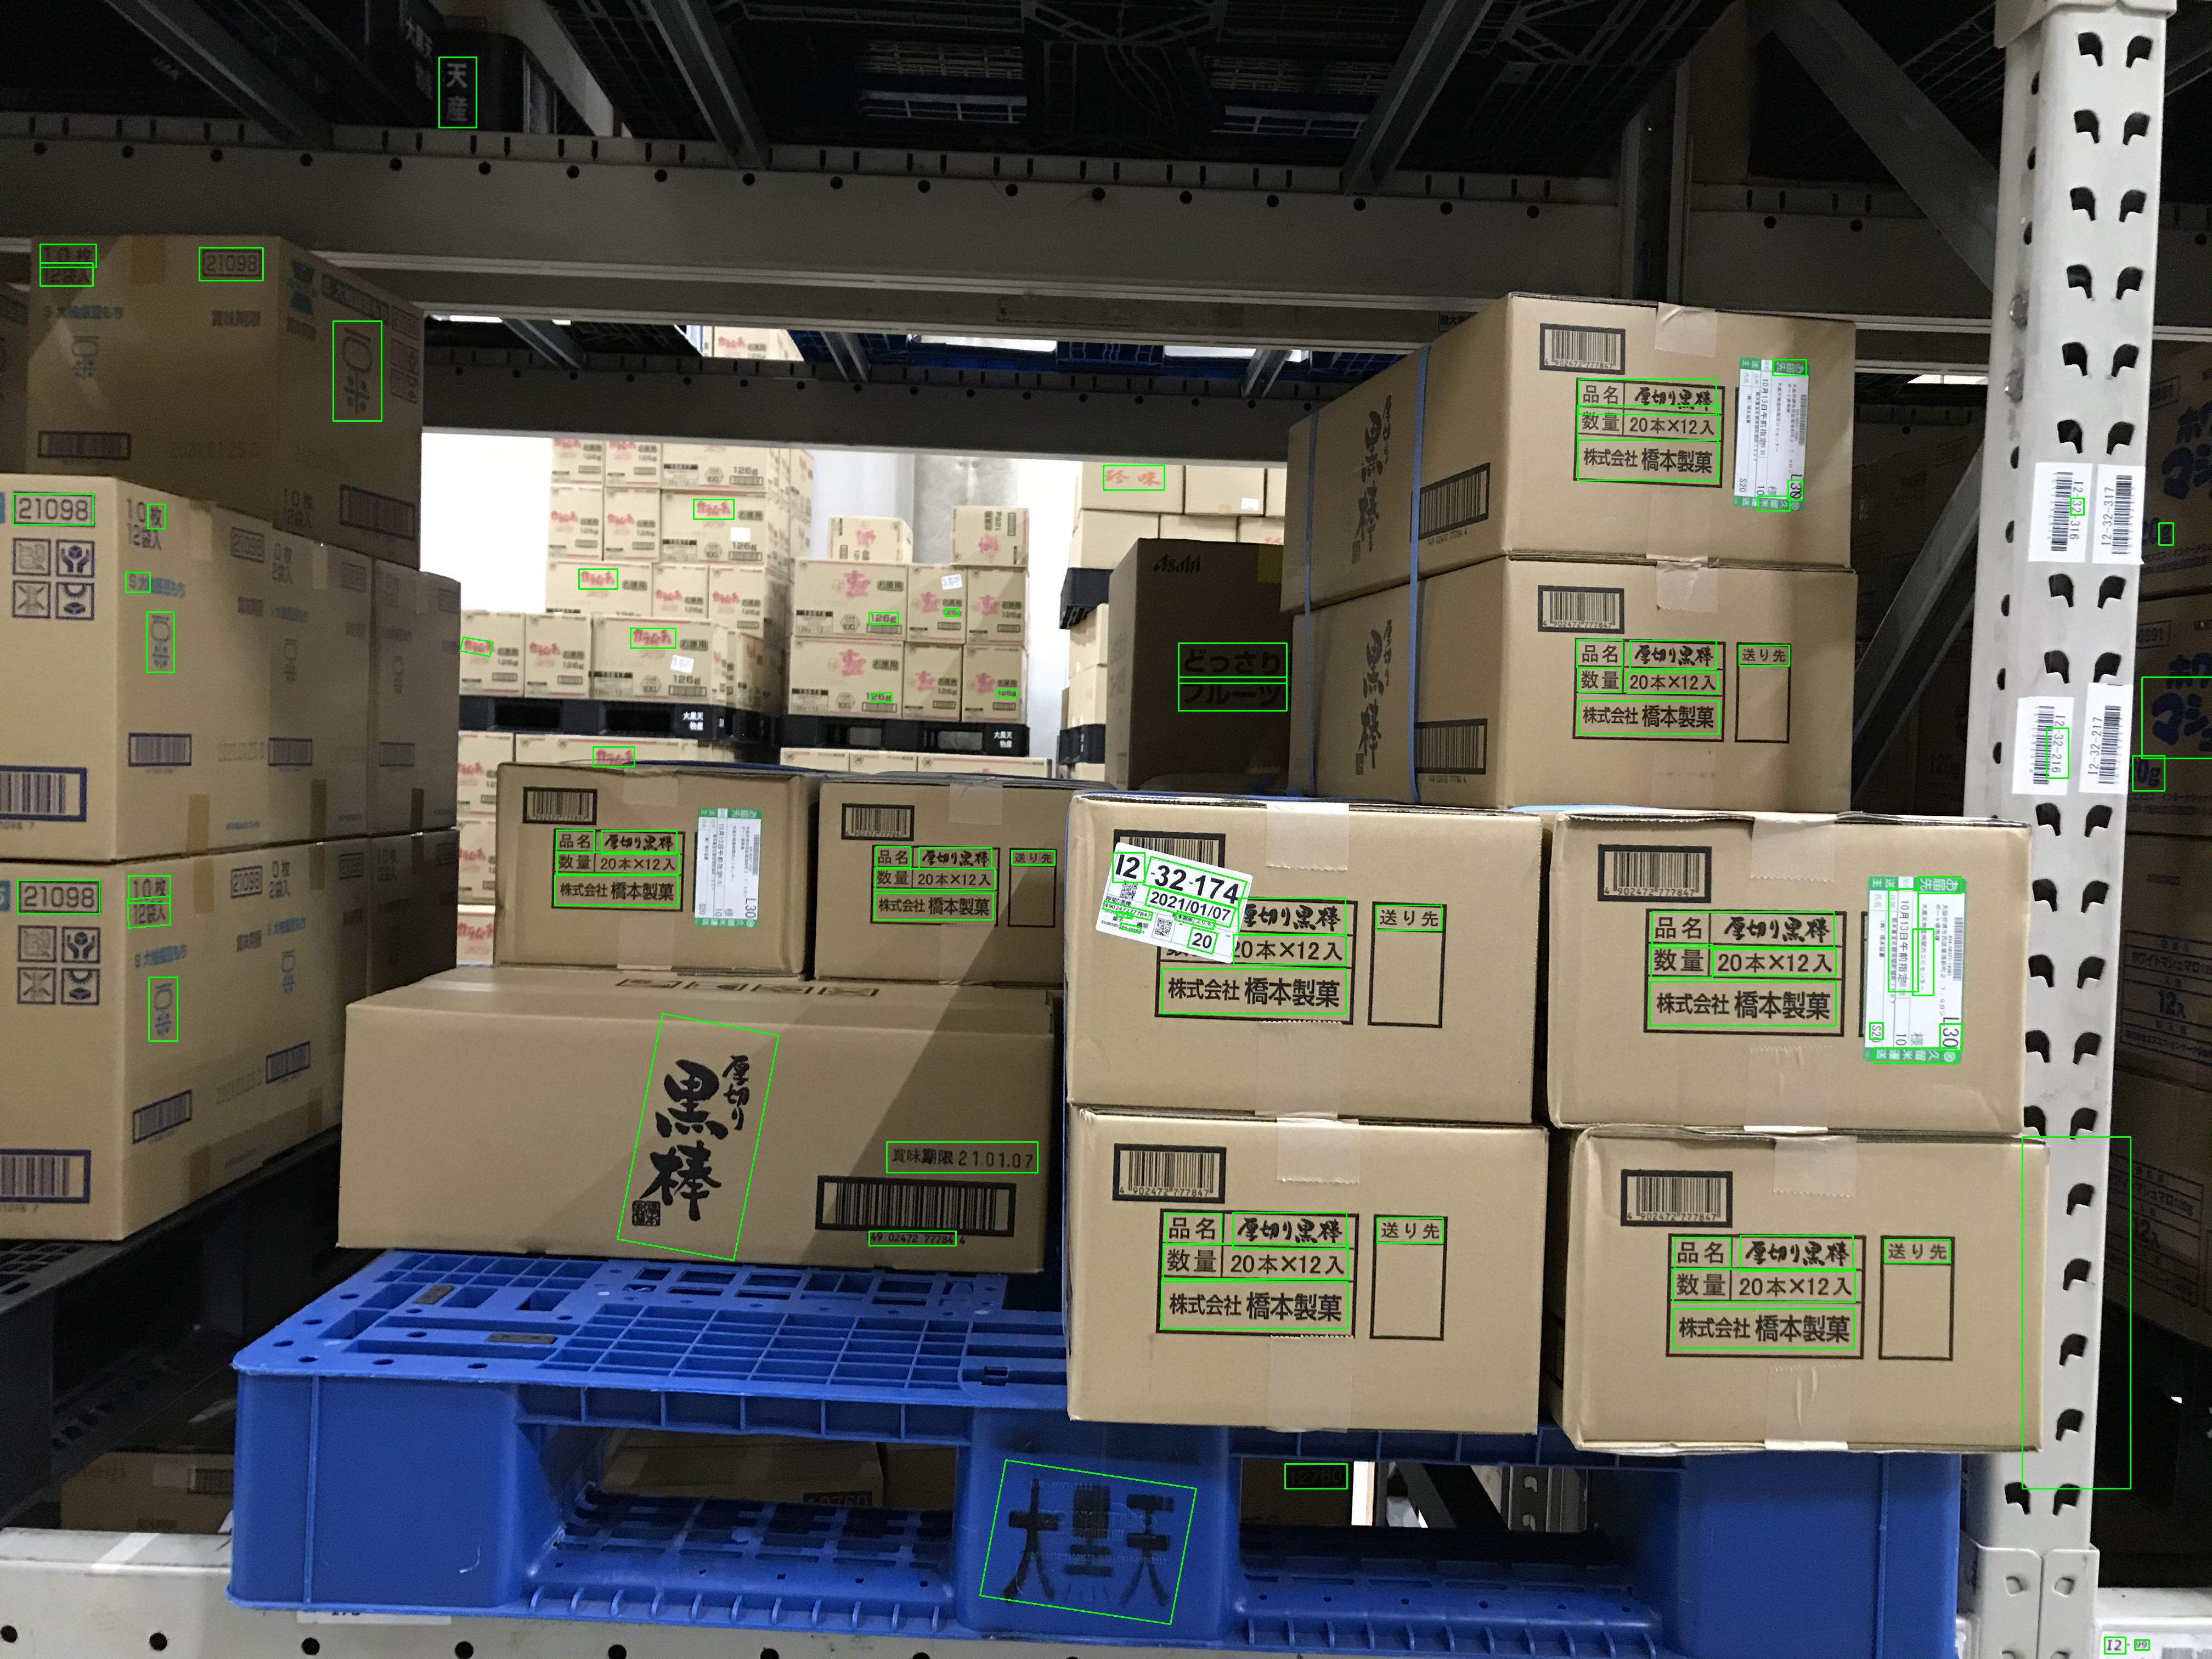
\includegraphics[width=0.8\columnwidth]{detection.png}  
   
	\caption{image after detection marked with green bounding boxes}
\end{figure}

\subsection{Date Text Filtering}

In the filtering part, we trained a binary classification model as ResNet-50 on the data-set provided by our cooperate company. this sub-set include 2 types of boxes, one is our target date boxes, and the other is no-date boxes which need to be removed from all the boxes. In fig.4, we present several boxes in filtering data-set which left is date and right is non-date.

\begin{figure}[ht] \centering    
	\label{filtering}     
	\includegraphics[width=0.8\columnwidth]{filter.png}  
   
	\caption{date boxes (left) and non-date boxes (right) in filtering dataset}
\end{figure}

The classifier has been well trained so that we could filter the useless texts from our crops get from the second step.

\subsection{Date Recognition}

Once we finished filtering the boxes and get only the date images, We will use an deep learning model which name is STAR-Net and its pre-trained weight to recognize all the date images. To make the recognition process effective and accurate enough, a series of experiments has been set to modify the model here, we will introduce the details of experiment in the next section.\par
In this part, the date boxes would be translated into text consist of digital and punctuation illustrated as Fig.5

\begin{figure}[ht] \centering    
	\label{recognition}     
	\includegraphics[width=0.8\columnwidth]{recognition.png}  
   
	\caption{date boxes (left) and recognition model outputs(right)}
\end{figure}

\subsection{Regular Expression Parsing(more explanation)}

In this part we generate the regular expression to parse our model outputs to dates, all the output of model will be transformed into an uniform format : Year Year Year Year/Month Month/Day Day.

Regular Expression is  used to standardize a canonical expression, and it has properties and methods to check whether the given string conforms to the rules.\par

\begin{figure}[ht] \centering    
	\label{parsing}     
	\includegraphics[width=0.8\columnwidth]{parsing.png}  
   
	\caption{recognition model outputs(right) and date after regular expression parsing}
\end{figure}

\subsection{Result Aggregation(more explanation)}

In our dataset, there are some images appear several times corresponding to a same ground-truth dates and index, so we need to select a highest repetition result as the only output for those images

\begin{figure}[ht] \centering    
	\label{aggregation}     
	\includegraphics[width=0.8\columnwidth]{aggre.png}  
   
	\caption{aggregate several repeat outputs to one}
\end{figure}

\section{Experiments}

To built a high accuracy Scene Text Recognition system, we set a series of experiments to modify each part inside our pipeline. 

\subsection{Experiment Environment}

We simply use 4 GTX 1080Ti GPUs with 12 GBs for pre-training and fine-tuning. For the OCR models, the batch size is all set to 192, the optimizer, learning rate, loss function. For the filtering models....(Maybe present this part in a table is better?)

\subsection{Filtering model Training}

In this part, our goal is to remove the non-date images from all of the cropped images that are processed in the detection part. To archive this goal, we train a binary classifier specifically to do this filtering. Here we choose ResNet-50 as the main architecture. 

Fig.7 is the evaluation accuracy curve of classifier. the final result archived 99.8%

\subsection{Date Recognition Experiments}

2parts: 1. setting a series of experiments to choose the best baseline model.
2. recognition with or without punctuation and CTC or Attn.\par

Introduce the definition of Separator and corresponding separator strategy.\par

Fig.8 is the bar plot of several baseline model: x axis is E-OCR, Rosetta, STAR-Net, and y axis is accuracy.\par

Table.2 accuracy of different combination with prediction module and separator strategy.

\subsection{Error Analysis}

Present the plots of different types of errors and analyze them separately. 
1. Pattern Error
2. Invalid Date 
3. blur images difficult to recognize
4. Ground-truth error.\par

Fig.9 present images of 4 types error and their labels

\subsection{Proposed Method}

Some errors(Error type.1 and type.2) outputed by the model do not correspond to the valid date(2021.11.37)  , by given a correctly defined regex, the model can exclude such prediction from the set of possible output. and output the highest probability sequence that matches the regular expression.\par

Table.3 Here illustrates the fixed errors

\section{Related work(unfinished)}

details of traditional OCR system \par
introduction of What Is Wrong With Scene Text Recognition Model Comparisons

The paper What is wrong with xxxx provide us an effective framework to evaluate most of the existing STR model.

Transformation is a module to translate all the original images into normalized images. The text in the actual scene images usually appears in various shapes  such as curved and slanted, the different shapes of texts will cause the following part more difficult to extract the feature from the original image. So the thin-plate spline (TPS) transformation, a variant of the spatial transformation network (STN), has been implemented in the first part of the OCR model. the image after TPS process would be shown as Fig.5 

Fig.5 a curved image as the input of TPS, and a normalized image as the output. 

In the Feature Extraction stage, a CNN like ResNet would be used to extract the feature map from the normalized image getting from TPS. These features are used to estimate the character on each receptive field.

Then in the Sequence model stage, The STAR-Net used BiLSTM to reshape the extracted features from the second stage to be a sequence of features, each column in a feature map is used as a frame of the sequence. The Bidirectional structure could solve the problem like the lack of contextual information.

The last stage: Prediction. The STAR-Net provided 2 options for choosing, Contortionist temporal classification (CTC) and attention-based sequence prediction (Attn). However, the pre-trained weight they provided, only the Attn could recognize the punctuation like ',' or '.'. Due to the data we have was in the type of date, which include many punctuation and Japanese characters, we choose the Attn as the set of Prediction Stage.

\section{Conclusion and Future work}

In this paper, we present our pipeline, an combination of several deep learning models for recognizing the structure text in the actual scenes. Currently existed STR model did not provide a effective method to recognize the structure text, so we set ourselves a goal to develop a pipeline that could help users to extract the target structure text information from images with complicated environment and translated the text into uniform format. Our pipeline consist of 5 parts to do the STR task: Detection and filtering help users to extract the target texts boxes from original image, Date Recognition translate the target boxes into computer text format, finally the Parsing and Aggregation would transform kinds of different texts into uniform format and choose the correct one as the final output. Experiments results show that our pipeline has archived a pretty good accuracy based on our dataset. We believe that this pipeline could help both the users and researchers in the Scene Text Recognition (STR) field.

For future research, we will constantly modify our pipeline to improve the accuracy, such as replace the backbone OCR model by Tr-OCR, a current State-of-the-art Transformer-based OCR model for text recognition.

For lack of a common dataset of structure text, we also welcome other researchers in this field to use and comment on our pipeline, and we will continue to improve our pipeline to address those issues.


% References should be produced using the bibtex program from suitable
% BiBTeX files (here: strings, refs, manuals). The IEEEbib.bst bibliography
% style file from IEEE produces unsorted bibliography list.
% -------------------------------------------------------------------------
\bibliographystyle{IEEEbib}
\bibliography{icme2020template}

\end{document}
